\documentclass[border=4pt]{standalone}
\usepackage{amsmath,amssymb}
\usepackage{tikz}
\usetikzlibrary{positioning,arrows.meta,calc,decorations.pathmorphing,fit}
\definecolor{newbg}{RGB}{255,255,255}
\begin{document}
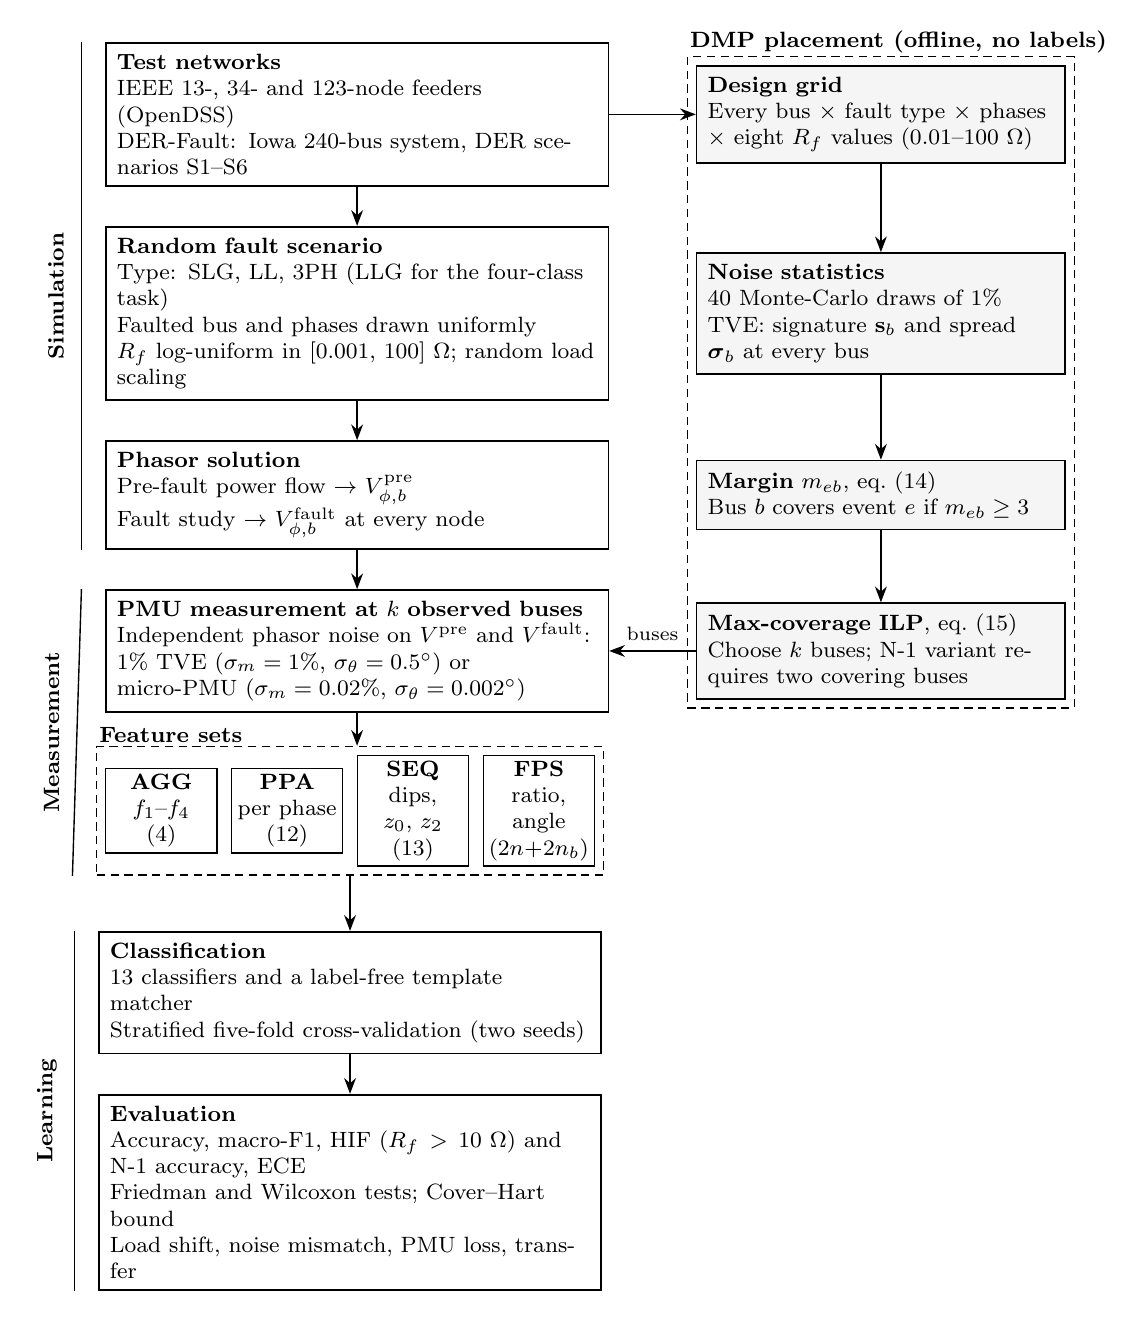
\begin{tikzpicture}[
  font=\footnotesize,
  node distance=5mm,
  main/.style={draw, line width=0.6pt, fill=white, align=left, text width=6.1cm, inner sep=4pt},
  side/.style={draw, line width=0.6pt, fill=gray!8, align=left, text width=4.4cm, inner sep=4pt},
  feat/.style={draw, line width=0.5pt, fill=white, align=center, text width=1.27cm, minimum height=1.0cm, inner sep=2pt},
  arr/.style={-{Stealth[length=2mm]}, line width=0.6pt},
  hd/.style={font=\footnotesize\bfseries},
  stage/.style={font=\footnotesize\bfseries, rotate=90, anchor=south}
]
% ---------------- main chain (top to bottom)
\node[main] (net) {\textbf{Test networks}\\
  IEEE 13-, 34- and 123-node feeders (OpenDSS)\\
  DER-Fault: Iowa 240-bus system, DER scenarios S1--S6};
\node[main, below=of net] (scen) {\textbf{Random fault scenario}\\
  Type: SLG, LL, 3PH (LLG for the four-class task)\\
  Faulted bus and phases drawn uniformly\\
  $R_f$ log-uniform in $[0.001,\,100]~\Omega$; random load scaling};
\node[main, below=of scen] (sim) {\textbf{Phasor solution}\\
  Pre-fault power flow $\rightarrow$ $V^{\mathrm{pre}}_{\phi,b}$\\
  Fault study $\rightarrow$ $V^{\mathrm{fault}}_{\phi,b}$ at every node};
\node[main, below=of sim] (pmu) {\textbf{PMU measurement at $k$ observed buses}\\
  Independent phasor noise on $V^{\mathrm{pre}}$ and $V^{\mathrm{fault}}$:\\
  1\% TVE ($\sigma_m=1\%$, $\sigma_\theta=0.5^\circ$) or\\
  micro-PMU ($\sigma_m=0.02\%$, $\sigma_\theta=0.002^\circ$)};
% feature sets as four parallel blocks
\node[feat, below=7mm of pmu.south west, anchor=north west] (f1) {\textbf{AGG}\\$f_1$--$f_4$\\(4)};
\node[feat, right=1.7mm of f1] (f2) {\textbf{PPA}\\per phase\\(12)};
\node[feat, right=1.7mm of f2] (f3) {\textbf{SEQ}\\dips, $z_0$, $z_2$\\(13)};
\node[feat, right=1.7mm of f3] (f4) {\textbf{FPS}\\ratio, angle\\($2n+2n_b$)};
\node[draw, densely dashed, line width=0.5pt, fit=(f1)(f4), inner sep=3pt,
      label={[hd, anchor=south west, inner sep=1pt]north west:Feature sets}] (fs) {};
\node[main, below=7mm of fs.south, anchor=north] (clf) {\textbf{Classification}\\
  13 classifiers and a label-free template matcher\\
  Stratified five-fold cross-validation (two seeds)};
\node[main, below=of clf] (ev) {\textbf{Evaluation}\\
  Accuracy, macro-F1, HIF ($R_f>10~\Omega$) and N-1 accuracy, ECE\\
  Friedman and Wilcoxon tests; Cover--Hart bound\\
  Load shift, noise mismatch, PMU loss, transfer};
\draw[arr] (net) -- (scen);
\draw[arr] (scen) -- (sim);
\draw[arr] (sim) -- (pmu);
\draw[arr] (pmu.south) -- (pmu.south |- fs.north);
\draw[arr] (fs.south) -- (clf.north);
\draw[arr] (clf) -- (ev);
% ---------------- DMP branch (offline, no labels)
\coordinate (bx) at ($(net.east)+(11mm,0)$);
\node[side, anchor=west] (grid) at (bx |- net.east) {\textbf{Design grid}\\
  Every bus $\times$ fault type $\times$ phases $\times$ eight $R_f$ values (0.01--100~$\Omega$)};
\node[side, anchor=west] (mc) at (bx |- scen.east) {\textbf{Noise statistics}\\
  40 Monte-Carlo draws of 1\% TVE: signature $\mathbf{s}_b$ and spread $\boldsymbol{\sigma}_b$ at every bus};
\node[side, anchor=west] (mg) at (bx |- sim.east) {\textbf{Margin} $m_{eb}$, eq.~(14)\\
  Bus $b$ covers event $e$ if $m_{eb}\ge3$};
\node[side, anchor=west] (ilp) at (bx |- pmu.east) {\textbf{Max-coverage ILP}, eq.~(15)\\
  Choose $k$ buses; N-1 variant requires two covering buses};
\node[draw, densely dashed, line width=0.5pt, fit=(grid)(ilp), inner sep=3pt,
      label={[hd, anchor=south west, inner sep=1pt]north west:DMP placement (offline, no labels)}] (dmp) {};
\draw[arr] (net.east) -- (grid.west);
\draw[arr] (grid) -- (mc);
\draw[arr] (mc) -- (mg);
\draw[arr] (mg) -- (ilp);
\draw[arr] (ilp.west) -- node[above, font=\scriptsize] {buses} (pmu.east);
% ---------------- stage labels
\draw[line width=0.5pt] ([xshift=-3mm]net.north west) -- ([xshift=-3mm]sim.south west)
  node[midway, stage, xshift=0mm, yshift=1mm] {Simulation};
\draw[line width=0.5pt] ([xshift=-3mm]pmu.north west) -- ([xshift=-3mm]fs.south west)
  node[midway, stage, yshift=1mm] {Measurement};
\draw[line width=0.5pt] ([xshift=-3mm]clf.north west) -- ([xshift=-3mm]ev.south west)
  node[midway, stage, yshift=1mm] {Learning};
\end{tikzpicture}
\end{document}
